\section{System Implementation}

In this section we describe a straight-forward implementation of \projname{} -- a distributed shared memory system implemented entirely in user-space.

\subsection{Overview}
In section \ref{vmm-design} we discussed a rudimentary design for the virtual memory manager which addressed problems like address space utilization and synchronization.  In section \ref{network-stack-design} we discussed the need for several in-process network daemons.  One design requirement that is the same from both of these sections is that there must exist a clean separation of the following: process-specific memory, shared memory and application memory.  The following is a list and summarization of the different types of memory that may exist in a target-application linked with the \projname{} library.

\begin{description}
\item[Process-specific Memory] \hfill \\
Any memory that is unique to a \projname{} node is considered process-specific memory.  Memory of this nature is kept separate from other types of memory, and is not subject to synchronization or change from any other node.  An example of this type of memory is for the network daemons.  The network daemons' call stacks and heaps must be unique per process because each node is running their own network stack.  The best way we found to ensure that other nodes do not interfere with this memory is to mantain a process-specific region of memory.

\item[Shared Memory] \hfill \\
Any memory that should be shared between \projname{} nodes is considered shared memory.  Memory of this nature should ideally be identical between all nodes in the cluster.  An example of this type of memory is the page table and other data structures used to maintain page ownership and location.

\item[Application Memory] \hfill \\
Any memory that is allocated or used by the target-application is considered application memory.  This is the memory that one uses when using \verb,malloc, within a normal application.  This memory is distinct from \projname{}-specific memory in that \projname{} \em manages \em the application memory.  Application memory need not exist on all nodes at all times, but it must be accessible to all nodes at all times.
\end{description}

Maintaining a clean separation of the different types of memory makes implementing the SDSM system significantly easier for the reasons described in section \ref{vmm-design}.  We implemented this requirement by allocating and managing fixed regions of memory in the process address space as depicted in figure \ref{process-structure}.  General-purpose use of these fixed regions of memory required custom allocators built to manage memory over these fixed regions.  We opted to use \em heap layers \em to construct these allocators.  Hoard and \em heap layers \em are discussed in greater detail in future sections.

\begin{figure*}[t]
\centering
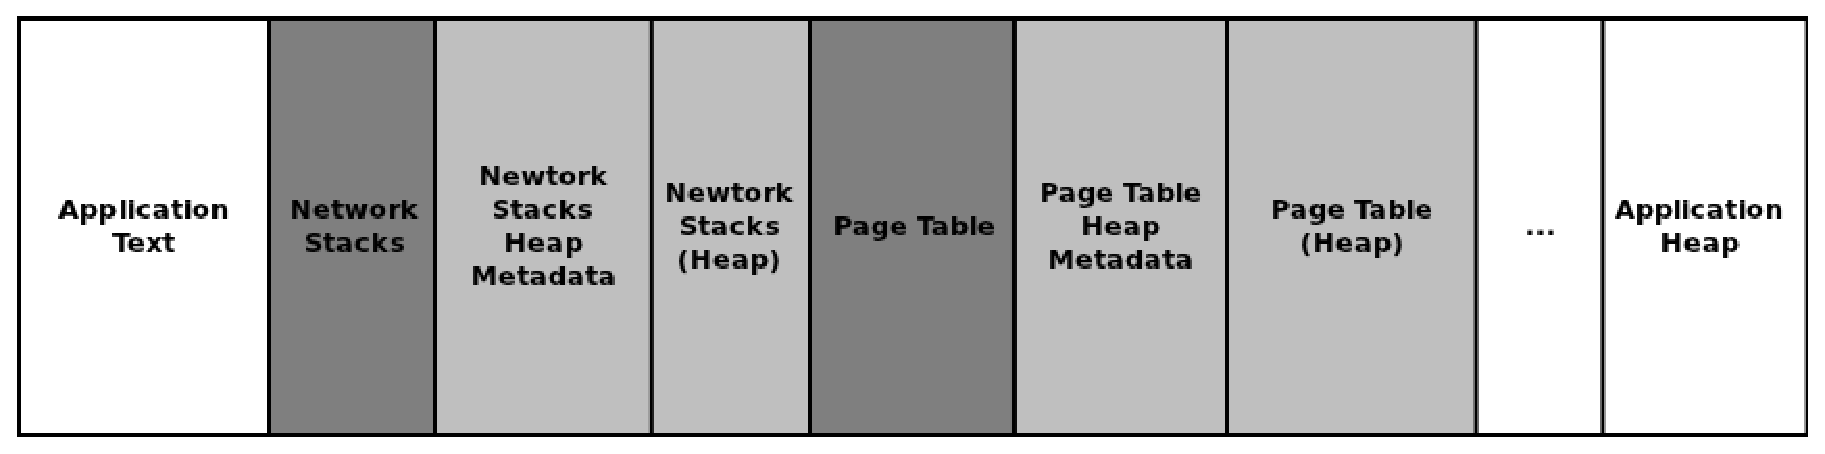
\includegraphics[scale=0.40]{images/process-structure.eps}
\caption{The \projname{} process structure.}
\label{process-structure}
\end{figure*}

\subsection{Virtual Memory Management}
The virtual memory manager is the soul of the \projname{} system.  It understands and coordinates the events that drive the network stacks, and is the primary data structure that coordinates the cluster.  At the heart of the VMM resides Hoard~\cite{Berger:1999:HFS:899944, Berger:2000:HSM:356989.357000}: a fast, scalable, and memory-efficient allocator for shared-memory multiprocessors.  The VMM is the primary source of events in the system, that are communicated to other nodes via the network stacks.

The following subsections discuss Hoard, the VMM used by \projname{}, and the process of resolving various types of page faults.

\subsubsection{Hoard}
VanHilst and Notkin introduced an implementation of \em collaboration-based \em designs that used C++ templatized class inheritance known as \em mixins\em~\cite{Smaragdakis:2000:MPC:645417.652070}.  Compared to other techiniques, their method yields less redundant and reusable components.  The standard approach to build components that exhibit a collaboration-based design in C++ use virutal method calls at each abstraction boundary~\cite{Berger:2002:MMH:997313}.  The cost of virtual method dispatching cannot be overlooked in high-performance applications, as is the case for memory allocators in which the cost of dispatching virtual functions is significant to the cost of allocating memory.  Using a mixin design, one avoids the cost of virtual method dispatch entirely.  Despite the highly efficient design, C++ mixins are not without cost.  The first users of C++ mixins rebuked it as a difficult design paradigm to understand~\cite{Smaragdakis:2000:MPC:645417.652070}.  The users went so far as to say that the design paradigm might not scale well because the layers can become so complex.

C++ mixins follow the exhibit the following design pattern.  Typically, a mixin body calls its superclass's version of the same method, adding an instrumentation layer over the method rather than overriding it entirely.

\begin{verbatim}
template <class Super> 
class Mixin : public Super {
  ... /* mixin body */
};
\end{verbatim}

Emery Berger introduced \em heap layers \em in \cite{Berger:2002:MMH:997313}.  Heap layers use a C++ mixin design to compose layers of allocators -- each layer adding functionality to \verb,malloc, or \verb,free,.  This design features highly reusable components that can be used as building blocks to compose other memory allocators.  For example, most heap layers inherit from what Berger called a \em source heap \em like \verb,MmapHeap,.  This heap is responsible for allocating chunks of memory from the operating system.  This layer can be specialized by wrapping it in addition layers -- perhaps \verb,FreelistHeap, or \verb,FirstFirstHeap,.

% TODO: page 46 of Berger's PhD thesis.  Talk more about it here.  Include code.

Hoard is memory management layer that uses a set of heap layers to provide a fast, efficient and scalable memory allocator.  It is a shared library that replaces the system provided allocator (e.g., \verb,malloc, and \verb,free,) with its own implementations that draw memory from its own allocatored composed of heap layers.  Hoard was a natural starting point for the implementation of \projname{} because it provided all of the necessary infrastructure for building a SDSM system: system hooks to replace malloc and a primary allocator constructed with replacable memory allocators.

The \projname{} system implements a special heap layer used for allocating memory.  This allocator is responsible for maintaining a global address space.  The heap layer we introduced is a \em source heap\em -- it is the interface between the application program and the operating system.  Before any node allocates memory, the underlying operating system is made aware of virtual memory mappings on all nodes in the cluster.  This way, new memory mappings will never conflict with existing mappings on a different node.  Additionally, when new mappings are introduced, internal data structures can be udpated and distributed to other nodes in the cluster.  The internal data structures used by this heap layer is the subject of the following section.

In addition to providing new heap layers for the \projname{} system's global address space, we introduced new heap layers for the data structures that maintain the global address space.  The C++ standard template library provides many helpful data strutures that can be paramaterized with a custom allocator.  We added heap layers to act as custom STL allocators.  The use of these allocators will become more apparant in the following sections.

\subsubsection{Page Table}
In traditional systems a virtual memory system is powered by a data structure called a page table.  The page table maintains mapping between a process's virtual address space and the underlying physical pages managed by the kernel.  The data structures that power the \projname{} system were inspired by this traditional design, but differ slightly only in implementation.  The \projname{} system's data structure resembles a traditional page table in that it maintains what virtual memory has been allocated in the system.  However, instead of mapping virtual pages to physical pages, the system maps virtual pages to internet addresses.  Each internet address indicates the current owner of that page.

The primary data structure used in \projname{} has the following \verb,std::map, type.  The data structure maintains a virtual address to a tuple containing pointers to \verb,Page, and \verb,Machine, objects, respectively.  These objects maintain metadata about the items they represent.  For virtual pages, this metadata includes the address, page protection bits, a page dirty bit and lastly, a version.  For machines, this metadata includes the internet address and a status enumeration indicating what the machine is currently doing.

\begin{verbatim}
typedef
std::pair<Page*,  Machine*> PTElement;

typedef
std::map<vmaddr, PTElementType,
      std::less<vmaddr>,
      PTAllocator<
        std::pair<vmaddr, PTElement> > >
          PTable;
\end{verbatim}

The \projname{} page table is instantiated in a fixed location -- see figure \ref{process-structure} -- using placement new.  The \verb,PTAllocator, is a special allocator composed of a \verb,FirstFitHeap, wrapped over a \verb,MmapHeap, type.  The allocator ensures that all memory allocated by the \verb,std::map, object resides in the fixed region of memory designated for the page table's heap.  As a result, the \verb,std::map, object and its associated heap reside in a fixed and known location in memory.

The most convenient feature of this design is the minimal amount of effort required to instantiate the same \verb,std::map, object on $n$ many nodes.  For example, after instantiating an object of type \verb,PTable, -- presumably on the master node -- one must simply copy this memory from one node to another.  After memory is copied from the master node to a worker node, the worker node need only cast the new memory region as a \verb,PTable,.  At this point, the worker can use the \verb,std::map, object as if it had instantiated the object itself.

Synchronizing the entire page table region is a heavyweight operation that requires locking and significant network communication overhead.  At the very least, the operation involves transmitting roughly six pages (4096 bytes) of memory.  Therefore, synchronizing the entire page table region is typically done very infrequently.  Special care is taken when using the page table to ensure that write operations are done by the master.


\subsubsection{Fault Handling}
At this point, we have established how we have instantiated a global address space.  Once a node is made aware of memory mappings of other nodes via synchronizing its page table memory region with the master's, the act of looking up who owns a memory mapping is as simple as executing a call to \verb,std::map::find, with the page-aligned address.  The result is a tuple containing pointers to \verb,Page, and \verb,Machine, objects respectively.  Using this metadata, one node may communicate with the current owner of a memory page.

We register a signal handler for the \verb,SIGSEGV, signal during initialization code that bootstraps the \projname{} system.  This signal is generated upon an illegal memory access either because the offending instruction is accesses memory that has not been allocated in the process's address space or because the memory protections on that page forbid access to it.  Access, in this case, can refer to \em read\em, \em write\em, \em execute \em or any combination of the above.  Upon receiving a \verb,SIGSEGV, signal, one may examine the \verb,siginfo_t, data to discover what address the instruction attempted to access.  One may use this address as a key into the page table to fetch the metadata for the page.  If no mapping exists, the signal exits the program -- this is a real segmentation violation.  If a mapping exists, this means that the address refers to a valid memory page in the cluster.

If a valid memory page exists in the cluster, it can exist on the faulting node or on another node available on the network.  In the former case, the node may only have read-only access to the page.  In the latter case, the node may be trying to access memory that it did not allocate locally.  In either case, the signal handler has all the information necessary to resolve the fault.  In the former case, the signal handler need only set memory protections to resolve the fault.  This case will likely set the page's dirty bit, so that changes can be propagated to other nodes at a future synchronization point.  In the latter case, the node may initiate a network transaction to download the page from the current owner.  This case involves communicating with the central manager to register the ownership change.

After the fault is resolved,  the offending instruction can be re-executed.

\subsection{Cluster Coordinator}
\label{cluster-coordinator}

The \projname{} system features several networking daemons to power the SDSM system.  These daemons include two network servers consisting of listeners for unicast and multicast traffic and two network clients consisting of speakers for unicast and multicast traffic.  The speakers are powered by a pool of threads and a work queue.  This work queue is a data structure populated by event handling code in the system.  For example, as discussed in previous sections, new definitions of \verb,malloc,, \verb,free,, and \verb,pthread, library functions usually push work onto these work queues.  These networking facilities provide a solid foundation for distributing messages and passively communicating with other nodes of the cluster.

We found that passively communicating certain events in the system was insufficient for maintaining a global address space.  These events include those like handing a fault or allocating new memory in the global address space.  We found that for these events, a blocking form of communication was necessary.  To accomodate this requirement, we added a networking suite that allowed blocking events to spawn a new network listener and speaker, this time one capable of blocking.  This new listener and speaker can block until a fault is resolved or an acknolwedgement is received without blocking the primary network stacks.

\subsubsection{Bootstrapping}

Bootstrapping the cluster was a non-trivial problem.  We shyed away from complicated configuration and manifest files by implementing multicast listeners in each of the nodes.  This multicast listener was capable of auto-detecting other nodes in the cluster with a heartbeat.  Upon joining the cluster, a centralized manager welcomes the new node with a three-way handshake.  Upon successful completion of the handshake -- which involves verification of the joining node's address space -- the joining node is sent the current version of the page table region.  Afterwards, the new node is ready to receive work.

\subsection{Threading}
One of those important feature of the \projname{} system are the new definitions provided for the \verb,pthread, library.  These features alone are the sole source of important \em events \em in the system.  This section is a discussion of each of the functions replaced.  Lastly, we discuss how these functions can be used to implement new memory coherence models in SDSM systems.

\begin{description}
\item[pthread\_create] \hfill \\
By intercepting and replacing \verb,pthread_create, we were able to prevent new threads from being created locally -- presumably on the master node -- and instead send a message to a remote node to create the thread there.  This was possible because the remote node shared an identical address space.  The loadable segment that matters in this case is the \verb,.text, section which holds all of the process's executable code.  Because this segment is identical, a function pointer can be passed in the message.  The receiving node can use this function pointer to create a local thread using \verb,clone(2),.  A thread identifier is returned to the node who issued the create message.  Any memory pages that this thread illegally accesses during exeuting will be faulted to the local node running the thread.

\item[pthread\_join] \hfill \\
By intercepting and replacing \verb,pthread_join, we were able to prevent a parent thread from continuing to execute until all children threads have been waited for.  This event causes the master thread to send a message to the node executing this thread.  The node can be discovered by querying local data structures that maintain a mapping of thread identifier to internet address.  The child node -- the one executing the thread -- can then call the real \verb,waitpid, call to wait for the \verb,clone(2), thread.

\item[pthread\_mutex\_init] \hfill \\
Though not necessary, we found that intercepting and replacing \verb,pthread_mutex_init, was convenient for building data structures on the central manager.  When a mutex is initialized, a message can be sent to the centralized manager notifying it that a new mutex has been created.  The address of this mutex can then be stored and used by the central manager -- or master -- to lookup future requests to that mutex.  We assume that properly written \verb,pthread, applications initialize any mutex variables with \verb,pthread_mutex_init,.

\item[pthread\_mutex\_lock] \hfill \\
By intercepting \verb,pthread_mutex_lock, we were able to send messages to the centralized manager requesting lock access to a mutex variable.  This call blocks until the lock has been granted.  This function has special semantics in regard to the coherency protocol.  The handling of this function is explained in greater detail in section \ref{coherency-protocol}.

\item[pthread\_mutex\_unlock] \hfill \\
By intercepting \verb,pthread_mutex_unlock, we were able to send messages to the centralized manager indicating that a thread no longer needs lock access to a mutex variable.  This call does not block.  This function has special semantics in regard to the coherency protocol.   The handling of this function is explained in greater detail in section \ref{coherency-protocol}.
\end{description}

\subsection{Coherence Protocol}
\label{coherency-protocol}

As previously mentioned, the handling of \verb,pthread_mutex_lock, and \verb,pthread_mutex_unlock, can be used to implement a lazy release consistency (LRC) coherency model.  This section is a discussion of how the \projname{} system implements this.

\subsubsection{Types}
\subsubsection{Architecture}

